\documentclass{beamer}

\mode<presentation>
{
  \usetheme{default}
  \usecolortheme{default}
  \usefonttheme{default}
  \setbeamertemplate{navigation symbols}{}
  \setbeamertemplate{caption}[numbered]
} 

\usepackage[english]{babel}
\usepackage[utf8x]{inputenc}

\title{Terminverwaltung App Projekt}
\author{Programmierung Java 2}
\date{09.07.2019}

\begin{document}

\begin{frame}
	\titlepage
\end{frame}

\section{Ziel}

\begin{frame}{Ziel}
	
	\begin{itemize}
		\item REST API Server als Backend für eine Web App
		\item Terminmanagement und Patientenverwaltung 
	\end{itemize}
	
	\vskip 1cm
	
	\begin{block}{Web App}
		Angular Projekt für Webaufbau - SS19
	\end{block}
	
\end{frame}

\section{Architektur}

\subsection{Web Server}

\begin{frame}{Web Server}
	
	\begin{itemize}
		\item Spring Boot
		\item Spring Framework + Embedded HTTP(s) Servers - XML Configuration
		\item Ökosystem von Spring (Spring ORM, Spring Security, ...)
	\end{itemize}
	
\end{frame}


\begin{frame}{Web Server}
	
	\begin{itemize}
		\item Tomcat als HTTP(s) Server
		\item Endpoints (Pfade):
		      \begin{itemize}
		      	\item /api/\{model\} \hspace{10mm} (GET/POST)
		      	\item /api/\{model\}/\{id\} \hspace{2mm} (PUT/DELETE)
		      \end{itemize}
		\item Request Type: "application/json"
		\item Response Type: "application/json"
		\item Authorization: Basic Auth
	\end{itemize}
	
\end{frame}


\subsection{Datenbank und ORM}

\begin{frame}{Datenbank}
	
	\begin{itemize}
		\item MySQL als Datenbank
		      \begin{itemize}
		      	\item MySQL Connector
		      \end{itemize}
		\item Spring Data JPA als ORM
		      \begin{itemize}
		      	\item Hibernate/JPA
		      	\item Entity, Repository, ...
		      \end{itemize}
	\end{itemize}
	
\end{frame}

\subsection{Modelle}


\begin{frame}{Modelle}
	
	\begin{itemize}
		\item User
		\item Patient
		\item Address
		\item Appointment
		\item AppointmentRecord
		\item Prescription
		\item Medicine
		\item ...
	\end{itemize}
	
	\vskip 1cm
	
	\begin{block}{Dokumentation}
		\href{https://termin-api.docs.stoplight.io/models}{- API Reference: Models}
	\end{block}
	
\end{frame}


\subsection{Beispiel}

\begin{frame}{Beispiel: /patient Endpoint}
	
	\begin{figure}
		\href{https://termin-api.docs.stoplight.io/patient-controller}{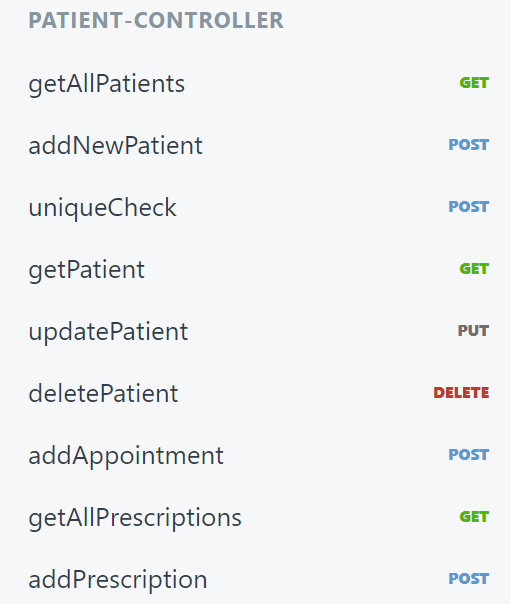
\includegraphics[width=60mm]{patient_endpoint.png}}
	\end{figure}
	
\end{frame}

\begin{frame}{Dokumentation}
	
	\begin{itemize}
		\item OpenAPI (Swagger) Spezifikation
		\item Standarte Dokumentationsnotation
	\end{itemize}
	
	\vskip 1cm
	
	\begin{block}{OpenAPI}
		- Hilft als offenes Beschreibungsformat dabei, den Überblick und das Verständnis über die Fähigkeiten eines API zu erhalten.
	\end{block}
	
\end{frame}

\begin{frame}{Automatisierte Dokumentation}
	
	\begin{itemize}
		\item Springfox - https://springfox.io
		\item Kontinuierliche Integration von Code und Dokumentation
	\end{itemize}
	
	\vskip 1cm
	
	\begin{block}{Springfox}
		\begin{itemize}
			\item Bietet die Integration von Swagger(OpenAPI) für Spring und Spring Boot Projekte.
			\item Überwiegend wird die Dokumentation aus den bereits vorhandenen Spring-Annotationen generiert.
			\item Swagger Annotation sind zusätzlich möglich.
		\end{itemize}
	\end{block}
	
\end{frame}

\begin{frame}{TODO}
	
	\begin{itemize}
		\item Weitere Validierung (Mehr als @NotNull)
	\end{itemize}
	
\end{frame}

\end{document}